% !Tex Program = xelatex
% -*-coding: utf-8 -*-
\documentclass[12pt,onecolumn]{report}

% 中文
\usepackage[BoldFont,SlantFont]{xeCJK}
\xeCJKsetemboldenfactor{1}%只对随后定义的CJK字体有效
\setCJKfamilyfont{hei}{SimHei}
\xeCJKsetemboldenfactor{4}
\setCJKfamilyfont{song}{SimSun}
\xeCJKsetemboldenfactor{4}
\setCJKfamilyfont{fs}{FangSong}
\setCJKfamilyfont{kai}{KaiTi}
\setCJKfamilyfont{li}{LiSu}
\setCJKfamilyfont{xw}{STXinwei}
\setCJKmainfont[BoldFont=SimHei]{SimSun}
\setCJKmonofont{SimSun}
\setCJKsansfont{SimSun}

\newcommand{\hei}{\CJKfamily{hei}}      % 黑体
\newcommand{\song}{\CJKfamily{song}}    % 宋体   (Windows 自带simsun.ttf)
\newcommand{\fs}{\CJKfamily{fs}}        % 仿宋体 (Windows 自带simfs.ttf)
\newcommand{\kai}{\CJKfamily{kai}}      % 楷体   (Windows 自带simkai.ttf)
\newcommand{\li}{\CJKfamily{li}}        % 隶书   (Windows自带simli.ttf)
\newcommand{\xw}{\CJKfamily{xw}}        % 隶书   (Windows自带simli.ttf)

% \AmSTeX\ 宏包,用来排出更加漂亮的公式。
\usepackage{amsmath}
% 定理类环境宏包,其中 \pkg{amsmath} 选项用来兼容 \AmSTeX\ 的宏包
\usepackage[amsmath,thmmarks,hyperref]{ntheorem}
\usepackage{amssymb}
% 添加字体
\usepackage[defaultsups]{newtxtext}
\usepackage{newtxmath}
\usepackage{courier}
% 图形支持宏包
\usepackage{graphicx}
% 插入pdf
\usepackage{pdfpages}
\includepdfset{fitpaper=true}
% 更好的列表环境。
\usepackage{enumitem}       %使用enumitem宏包,改变列表项的格式
\usepackage{environ}
% 禁止 \LaTeX 自动调整多余的页面底部空白,并保持脚注仍然在底部。
% 脚注按页编号。
\usepackage[bottom,perpage,hang]{footmisc}
\raggedbottom{}
% 脚注格式。
\usepackage{pifont}
% 表格控制
\usepackage{longtable}
\usepackage{booktabs}
% 参考文献引用宏包
\usepackage[sort&compress,numbers]{natbib}
% 生成有书签的 pdf 及其开关,请结合 gbk2uni 避免书签乱码。
\usepackage{hyperref}
\hypersetup{
  CJKbookmarks=true,
  linktoc=all,
  bookmarksnumbered=true,
  bookmarksopen=true,
  bookmarksopenlevel=1,
  breaklinks=true,
  colorlinks=false,
  plainpages=false,
  pdfborder=0 0 0}
% 设置 url 样式,与上下文一致
\urlstyle{same}
% 版芯设置
\usepackage{geometry}
\geometry{
  a4paper,
  centering,
  text={150true mm,236true mm},
  left=30true mm,
  head=5true mm,
  headsep=2true mm,
  footskip=0true mm,
  foot=5.2true mm
}
% 利用 \pkg{fancyhdr} 设置页眉页脚。
\usepackage{fancyhdr}
% 其他包,表格、数学符号包
\usepackage{tabularx}
\usepackage{varwidth}
% 此处changepage环境用来控制索引页面的左右边距,规范中给出的示例的边距要大于正文。
\usepackage{changepage}
% 多栏结构在文中用begin{multicols}{2}end{multicols}
\usepackage{multicol,multienum}
% 允许上一个section的浮动图形出现在下一个section的开始部分,还提供\FloatBarrier命
% 令,使所有未处理的浮动图形立即被处理
\usepackage[below]{placeins}
% 支持子图 %centerlast 设置最后一行是否居中
\usepackage{subfigure}
% 支持双语标题
\usepackage[subfigure]{ccaption}
% 根据我工规定,正文小四号 (12bp) 字,行距为固定值3--4mm。
\renewcommand\normalsize{
  \abovedisplayskip=8pt
  \abovedisplayshortskip=8pt
  \belowdisplayskip=\abovedisplayskip{}
  \belowdisplayshortskip=\abovedisplayshortskip}
% 根据习惯定义字号。用法:\cs{hit@def@fontsize}\marg{字号名称}\marg{磅数}避免了
% 字号选择和行距的紧耦合。所有字号定义时为单倍行距,并提供选项指定行距倍数。
\def\hit@def@fontsize#1#2{%
  \expandafter\newcommand\csname #1\endcsname[1][1.3]{%
    \fontsize{#2}{##1\dimexpr #2}\selectfont}}
\hit@def@fontsize{dachu}{58bp}
\hit@def@fontsize{chuhao}{42bp}
\hit@def@fontsize{xiaochu}{36bp}
\hit@def@fontsize{yihao}{26bp}
\hit@def@fontsize{xiaoyi}{24bp}
\hit@def@fontsize{erhao}{22bp}
\hit@def@fontsize{xiaoer}{18bp}
\hit@def@fontsize{sanhao}{16bp}
\hit@def@fontsize{xiaosan}{15bp}
\hit@def@fontsize{sihao}{14bp}
\hit@def@fontsize{banxiaosi}{13bp}
\hit@def@fontsize{xiaosi}{12bp}
\hit@def@fontsize{dawu}{11bp}
\hit@def@fontsize{wuhao}{10.5bp}
\hit@def@fontsize{xiaowu}{9bp}
\hit@def@fontsize{liuhao}{7.5bp}
\hit@def@fontsize{xiaoliu}{6.5bp}
\hit@def@fontsize{qihao}{5.5bp}
\hit@def@fontsize{bahao}{5bp}
% 利用 \pkg{enumitem} 命令调整默认列表环境间的距离,以符合中文习惯。
\setlist{nosep}
% 允许太长的公式断行、分页等。
\allowdisplaybreaks[4]
\predisplaypenalty=0  %公式之前可以换页,公式出现在页面顶部
\postdisplaypenalty=0
% 公式编号设置
\renewcommand{\theequation}{\arabic{chapter}.\arabic{equation}}
% 定理标题使用黑体,正文使用宋体,冒号隔开。
\theorembodyfont{\normalfont}
\theoremheaderfont{\normalfont\hei}
\theoremsymbol{\ensuremath{\square}}
\newtheorem*{proof}{证明}
\theoremstyle{plain}
\theoremsymbol{}
\theoremseparator{}
\newtheorem{assumption}{假设}[chapter]
\newtheorem{definition}{定义}[chapter]
\newtheorem{proposition}{命题}[chapter]
\newtheorem{lemma}{引理}[chapter]
\newtheorem{theorem}{定理}[chapter]
\newtheorem{axiom}{公理}[chapter]
\newtheorem{corollary}{推论}[chapter]
\newtheorem{exercise}{练习}[chapter]
\newtheorem{example}{例}[chapter]
\newtheorem{remark}{注释}[chapter]
\newtheorem{problem}{问题}[chapter]
\newtheorem{conjecture}{猜想}[chapter]
% 各种单位
\usepackage{siunitx}
\sisetup{group-minimum-digits=4, group-separator= \hspace{0.25em}}
\sisetup{detect-weight,detect-mode,detect-family}
% 处理数学公式中的黑斜体的宏包
\usepackage{bm}
% 不同于 \mathcal \mathfrak 之类的英文花体字体
\usepackage{mathrsfs}
% 支持彩色
\usepackage[table]{xcolor}
\definecolor{colorzero}{rgb}{0, 0, 0}
\definecolor{colorone}{rgb}{1, 0, 0}
\definecolor{colortwo}{rgb}{0, 0, 1}
\definecolor{colorthree}{rgb}{0, 1, 0}
% 图形和表格的控制旋转
\usepackage{rotating}
% 算法的宏包,注意宏包兼容性,先后顺序为float、hyperref、algorithm(2e),否则无法
% 生成算法列表。
\usepackage[algoruled,linesnumbered]{algorithm2e}
% 排版源码所使用的环境。
\usepackage{listings}
\lstset{
  language    = SQL,
  breaklines  = true,
  captionpos  = b,
  tabsize     = 2,
  numbers     = left,
  columns     = fullflexible,
  keepspaces  = true,
  frame       = shadowbox,
  commentstyle = \color[RGB]{0,128,0},
  keywordstyle = \color[RGB]{0,0,255}\bfseries,
  basicstyle   = \scriptsize\ttfamily,
  rulesepcolor = \color{red!20!green!20!blue!20},
  showstringspaces = false,
  breakatwhitespace = false,
}

% 作图
\usepackage{tikz}
\usetikzlibrary{graphs, positioning, quotes, shapes.geometric}

% 首行缩进
\usepackage{indentfirst}
\setlength{\parindent}{2em}

\usepackage{float}
\usepackage{diagbox}
\usepackage{setspace}
\usepackage{zhnumber}
\usepackage{titlesec}

% \renewcommand\thechapter{\zhnum{chapter}}
% \renewcommand\thesection{\arabic{section}}

\titleformat{\chapter}{\centering\Huge\bfseries}{第\,\thechapter\,章}{1em}{}
% \titleformat{\section}{\raggedright\Large\bfseries}{\thesection\,}{1em}{}
% \titleformat{\subsection}{\raggedright\large\bfseries}{\,\thesubsection\,}{1em}{}
% \titleformat{\subsubsection}{\raggedright\large\bfseries}{\,\thesubsubsection\,}{1em}{}

\graphicspath{{figures/}}
\bibliographystyle{plainnat}

\pagestyle{fancy}
\fancyhead[L]{\song\xiaowu[0]{cycleke}}
\fancyhead[C]{\song\xiaowu[0]{数据库实验一报告}}
\fancyhead[R]{\song\xiaowu[0]{哈尔滨工业大学}}
\fancyfoot[C]{\xiaowu-~\thepage~-}
\makeatletter
\def\headrule{{%
    \if@fancyplain\let\headrulewidth\plainheadrulewidth\fi
    \vskip2pt
    \hrule\@height2pt\@width\headwidth\vskip1pt
    \hrule\@height\headrulewidth\@width\headwidth\vskip-\headrulewidth\vskip-4pt
  }}
\makeatother

\fancypagestyle{plain}{
  \fancyhf{}
  \fancyhead[L]{\song\xiaowu[0]{cycleke}}
  \fancyhead[C]{\song\xiaowu[0]{数据库实验一报告}}
  \fancyhead[R]{\song\xiaowu[0]{哈尔滨工业大学}}
  \fancyfoot[C]{\xiaowu-~\thepage~-}
}

\renewcommand{\today}{\number\year{年}\number\month{月}\number\day{日}}
\renewcommand{\contentsname}{\centering \hei{目录}}
\renewcommand{\figurename}{图}
\renewcommand{\tablename}{表}
\renewcommand{\lstlistingname}{代码}
\numberwithin{figure}{chapter}
\numberwithin{table}{chapter}
\numberwithin{lstlisting}{chapter}

\renewcommand{\baselinestretch}{1.25}
\newcommand{\M}[1]{\mathbf{#1}}
\setcounter{secnumdepth}{4}

\begin{document}

\begin{titlepage}
  \vspace{5\baselineskip}

  \begin{figure}[H]
    \centering
    
\includegraphics[width=0.6\linewidth]{figures/school.eps}
  \end{figure}

  \centering\hei{}

  \xiaosan\vspace{\baselineskip}

  \makebox[150bp][s]{数据库实验一报告}

  \erhao\vspace{2\baselineskip}

  \makebox[300bp][s]{实验一:数据库设计与应用开发}

  \sanhao\vspace{3\baselineskip}

  \makebox[80bp][s]{姓名}~~\underline{\makebox[160bp][s]{c y c l e k e}} \\ [24pt]
  \makebox[80bp][s]{学号}~~\underline{\makebox[160bp][s]{x x x x x x x x x x}} \\ [24pt]
  \makebox[80bp][s]{老师}~~\underline{\makebox[160bp][s]{}} \\ [24pt]
  \makebox[80bp][s]{专业}~~\underline{\makebox[160bp][s]{计算机}} \\ [24pt]
  \makebox[80bp][s]{日期}~~\underline{\makebox[160bp][s]{2020 年 04 月 22 日}} \\ [24pt]
\end{titlepage}

\clearpage
\tableofcontents
\clearpage


\chapter{实验目的}
在本次实验中,
我需要构思一个规模合理且功能较完善的数据密集型应用场景,
之后根据应用需求设计一个关系数据库并开发数据库系统应用,
从而能够
\begin{enumerate}[fullwidth,itemindent=\parindent,label=\arabic*.]
\item 学会正确运用概念数据库设计方法,正确使用实体——联系图(ER 图)表示概念数据模型;
\item 学会正确运用逻辑数据库设计方法,在概念数据模型的基础上,设计合理的关系数据库模式;
\item 学会正确运用物理数据库设计方法,根据工作负载,合理设计数据库的存取方法与存储结构;
\item 掌握一种关系数据库管理系统(RDBMS)的使用方法,使用 SQL 创建、更新和查询关系数据库;
\item 掌握数据库系统应用开发方法。
\end{enumerate}

\chapter{数据库设计}
\section{需求分析}
在本次实验中,我计划设计一个书评管理系统。
在本书评系统中,
我们需要管理若干书籍以及书籍对应的评论
(包括书籍和评论的相关信息)。
在该系统中,具体的数据包括各种
书籍信息(包括书名、ISBN 码、书籍领域、作者和出版社),
出版社信息(包括出版社名称),
作者信息(包括姓名、性别),
评论信息(包括书籍、评论的读者和评论的内容),
读者信息(包括姓名)。

我们需要约束书籍的 ISBN 码各不相同,
书籍的领域在给定的若干个领域中,
其作者和出版社也必须是数据库中存在的实体。
作者的性别也必然是给定给定性别中的一种。
自然,评论的读者和数据也要在数据库中出现。

在使用书评系统时,
我们需要支持随时添加合法的
书籍、出版社、作者、读者和评论,
同时支持对于上述内容的搜索。
在搜索时,不同的内容支持不同的搜索方式。
如对于书籍,我们需要支持按照唯一的 ISBN 码来进行搜索,
对于评论、出版社等内容,我们需要支持按照评论内容是否包含给定的关键字来进行搜索。
为了便于管理,我们可以给每个实体设置一个编号,
自然书评系统需要支持按照编号进行搜索。

\section{概念数据库设计}

在书评系统中,
概念数据库的实体型包括出版社、书籍、作者和读者,
联系型包括出版关系、写作关系和评论关系。
其包含的属性值和关联实体如下:
\begin{itemize}[fullwidth,itemindent=\parindent]
\item 出版社:编号,名称;
\item 书籍:编号,ISBN 码,书名,领域;
\item 作者:编号,姓名,性别;
\item 读者:编号,姓名;
\item 出版关系:出版社,书籍;
\item 写作关系:作者,书籍;
\item 评论关系:编号,评论内容,读者,书籍。
\end{itemize}

根据上述的关系,我们可以画出对应的 ER 图,
之后分析实体之间的关系,是否有必要建立多元关系,再确定基数。
最终构造的 ER 图如图\ref{fig:ER-fig}。

\begin{figure}[ht]
  \centering
  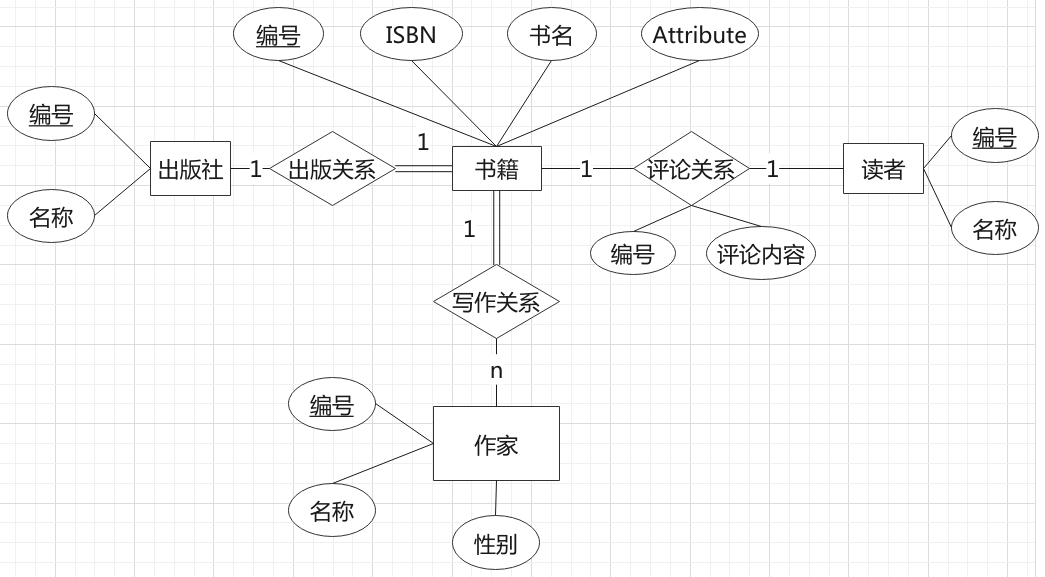
\includegraphics[width=\linewidth]{figures/er.png}
  \caption{概念数据库对应的 ER 图}\label{fig:ER-fig}
\end{figure}

\section{逻辑数据库设计}
由于出版关系仅与出版社和书籍相关,
且一个书籍仅与一个出版社存在该关系,
所以我将出版关系存储在书籍类中。
实体型转换的结果如下:
\begin{itemize}[fullwidth,itemindent=\parindent]
\item 出版社:Publisher (Id, Name)
\item 作者:Author (Id, Name, Sex)
\item 书籍:Book (Id, ISBN, Name, Category, PublisherId)
\item 读者:Reader (Id, Name)
\end{itemize}

关系型转换的结果如下:
\begin{itemize}[fullwidth,itemindent=\parindent]
\item 写作关系:WriteBook (AuthorId, BookId)
\item 评论关系:Comment (Id, ReaderId, BookId, Content)
\end{itemize}

\section{物理数据库设计}
对于绝大部分关系,
我使用其主键建立主索引
(写作关系的主键为 AuthorId 和 BookId 形成的二元组)。
在 MySQL 声明主键时,
系统会自动地建立主索引。
特别地,
我对于书籍上的 ISBN 还建立了一个唯一索引。

\section{数据库建立}
在本次实验中,
我使用 MySQL 来建立数据库。
其对应的 MySQL 代码为:
\begin{lstlisting}
CREATE TABLE Publisher (
  Id INT AUTO_INCREMENT PRIMARY KEY,
  Name VARCHAR(256) NOT NULL
);

CREATE TABLE Author (
  Id INT AUTO_INCREMENT PRIMARY KEY,
  Name VARCHAR(256) NOT NULL,
  Sex ENUM('男','女') NOT NULL
);

CREATE TABLE Book (
  Id INT AUTO_INCREMENT PRIMARY KEY,
  ISBN VARCHAR(17) NOT NULL UNIQUE,
  Name VARCHAR(20) NOT NULL,
  Category ENUM('社会科学', '自然科学', '文学', '技术', '军事', '宗教', '综合'),
  PublisherId INT NOT NULL,
  FOREIGN KEY (PublisherId) REFERENCES Publisher(Id),
  UNIQUE INDEX(ISBN)
);

CREATE TABLE Reader (
  Id INT AUTO_INCREMENT PRIMARY KEY,
  Name VARCHAR(256) NOT NULL
);

CREATE TABLE Comment (
  Id INT AUTO_INCREMENT PRIMARY KEY,
  ReaderId INT NOT NULL,
  BookId INT NOT NULL,
  Content VARCHAR(256) NOT NULL,
  FOREIGN KEY (ReaderId) REFERENCES Reader(Id),
  FOREIGN KEY (BookId) REFERENCES Book(Id)
);

CREATE TABLE WriteBook (
  AuthorId INT NOT NULL,
  BookId INT NOT NULL,
  PRIMARY KEY (AuthorId, BookId),
  FOREIGN KEY (AuthorId) REFERENCES Author(Id),
  FOREIGN KEY (BookId) REFERENCES Book(Id)
);
\end{lstlisting}

注意其中``关系型''对应的 MySQL 表中声明了外键,这样能够保证数据的一致性。

\chapter{数据库应用开发}
\section{数据库应用设计}
在本次实验中,
我将数据库管理同用户界面隔离,
这样便于后续数据库逻辑更改后应用的更新。
源代码的目录结构如下:
\begin{lstlisting}[language=bash]
src
|-- app.py
|-- data_manager
|   |-- author_manager.py
|   |-- book_manager.py
|   |-- comment_manager.py
|   |-- mysql_connect.py
|   |-- publisher_manager.py
|   |-- reader_manager.py
|   `-- write_book_manager.py
`-- ui
    |-- mainwindow.ui
    `-- ui_mainwindow.py

2 directories, 10 files
\end{lstlisting}

在开发应用的过程中,
我利用 PyMySQL 库来建立应用和 MySQL 数据库的连接,
使用 PyQt5 来实现图形化界面。

我将所有负责数据管理的类放置在 data\_manager 目录下,
其中 MySQLConnect 类负责管理同 MySQL 数据库的连接,
对一些重复率高的 MySQL 语句设置模版(如创建表、插入和查询语句)。
如对于插入数据,我使用格式化字符串来实现。
\begin{lstlisting}[language=python]
cursor.execute("INSERT INTO {} ({}) VALUES ({});".format(
    table, keys, values))
\end{lstlisting}

而 AuthorManager、BookManager、CommentManager、
PublisherManager、ReaderManager 和 WriteBookManager
分别管理作者表、书籍表、评论表、出版社表、读者表和写作关系表。
他们通过 MySQLConnect 类来连接连接数据库,
之后通过 MySQLConnect 类提供的 API 来
更新和查询自己负责的数据表,为前端程序提供数据的查询和更新。

同 GUI 界面相关的配置文件和界面配置则存放在 ui 目录下。
它们负责将数据直观地展示在用户面前,
同时为用户提供相应的输入和输出方式,
让用户能够通过一个简洁、友好的界面来对数据进行管理。

最后由 App 类负责将图形化界面同数据管理联系起来,
将相关的按钮和函数关联起来,实现让用户进行数据管理。

\section{实现结果}
在命令行中输入下面的指令即可运行该书评系统,
其初始界面如图\ref{fig:init}所示。
\begin{lstlisting}[language=bash]
python src/app.py
\end{lstlisting}

点击在出版社标签页中点击``列出所有''按钮,
应用会从数据库中获取所有的出版社信息并在表格中列出。
在其他的标签页中,
应用也提供相似的按钮来查看所有的相关信息。

\begin{figure}[ht]
  \centering
  \begin{minipage}{0.45\linewidth}
    \centering
    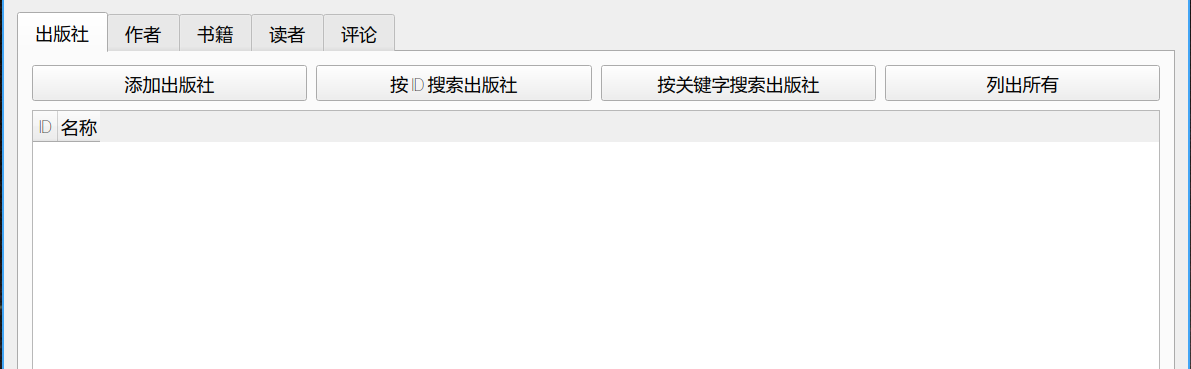
\includegraphics[width=\linewidth]{figures/init.png}
    \caption{应用初始界面}\label{fig:init}
  \end{minipage}
  \begin{minipage}{0.45\linewidth}
    \centering
    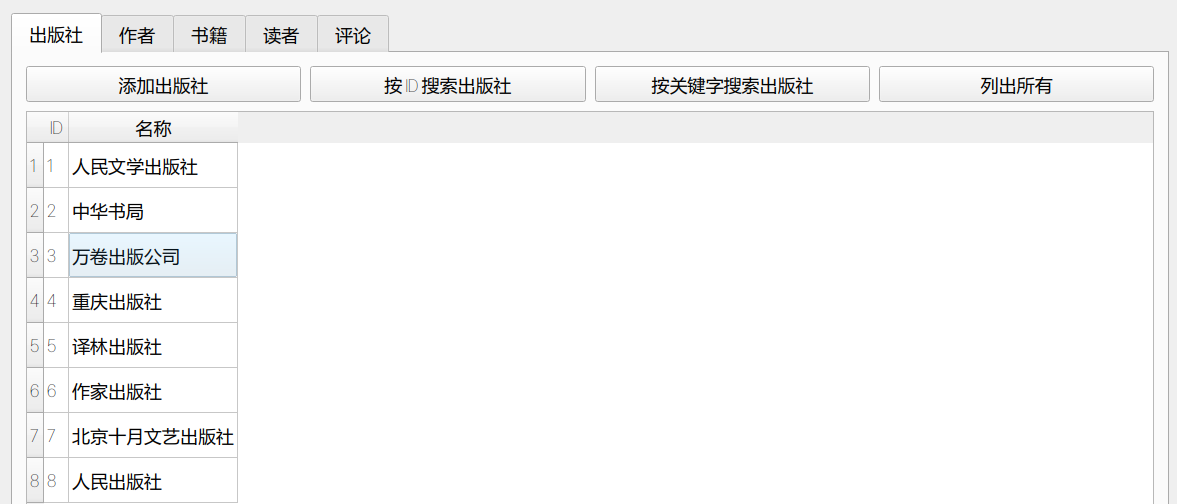
\includegraphics[width=\linewidth]{figures/publisher-list.png}
    \caption{列出所有出版社}\label{fig:publisher-list}
  \end{minipage}
\end{figure}

切换到评论页中,我们可以使用关键字搜索相关评论。
点击``按关键字搜索评论'',
应用会弹出输入关键字的搜索框(图\ref{fig:input-keyword}),
我们在其中输入``的''字,
表格中就会列出包含``的''字的评论(图\ref{fig:comment-list})。
对于其他数据,
应用还支持通过 ID 编号,ISBN,作者和读者等信息来进行搜索。

\begin{figure}[ht]
  \centering
  \begin{minipage}{0.45\linewidth}
    \centering
    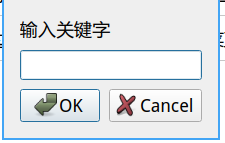
\includegraphics{figures/input-keyword.png}
    \caption{输入关键字}\label{fig:input-keyword}
  \end{minipage}
  \begin{minipage}{0.45\linewidth}
    \centering
    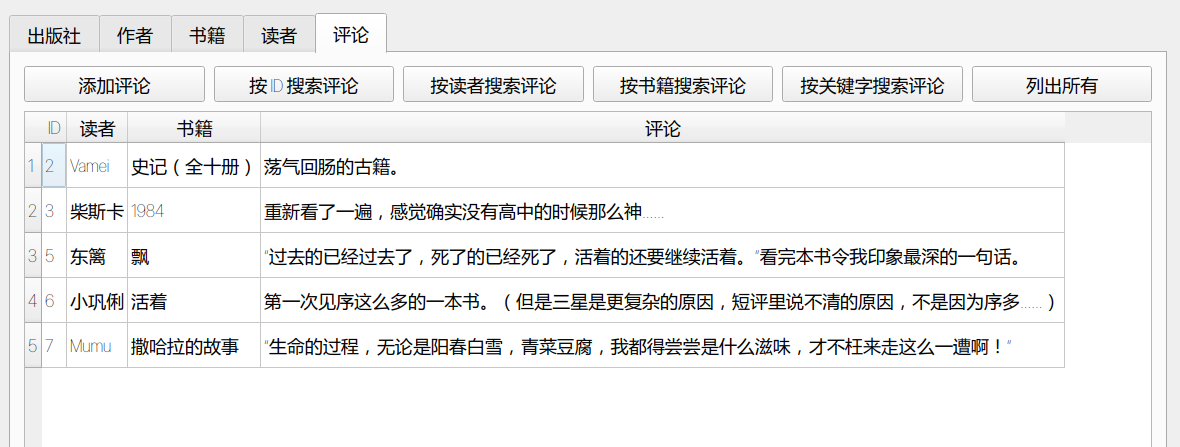
\includegraphics[width=\linewidth]{figures/comment-list.png}
    \caption{列出包含``的''字的评论}\label{fig:comment-list}
  \end{minipage}
\end{figure}

\chapter{实验总结}
在本次实验中,
我学会了正确运用概念数据库设计方法,
将概念数据库通过 ER 图形式化地表示出来,
并逐步转换为逻辑书籍库和物理数据库,
从而能够设计一个高效的关系数据库。
之后我利用设计初的数据库实现一个用户友好的数据库系统应用,
掌握数据库系统应用开发方法,
同时还提高了自己对于 MySQL 语言的熟悉程度。

\end{document}
